\chapter{Die MMU}

Die MMU (Memory Management Unit) verwaltet den in Bl\"ocke gegliederten Speicherbereich und die darauf erfolgenden Zugriffe. Die Einheit bietet dabei eine Schnittstelle für lesende und schreibende Speicheranfragen, welche in unterschiedlichen Zeitintervallen bearbeitet werden.

\section{\"Uberblick}

Der adressierbare Speicher innerhalb des Prozessors ist blockweise organisiert. Die MMU verwaltet einerseits die einzelnen Controller für die jeweiligen RAM-Bl\"ocke und taktet andererseits die angefragten Zugriffe auf diese.

Sie ist aufgrund der \"uberwiegend sehr \"ahnlichen Adressierungsprozeduren intern durch eine Statemachine realisiert, welche anhand einer Speicheradresse die jeweiligen Speicheranfragen an den dem RAM-Block entsprechenden Controller weiterleitet.

Um eine reibungslose Kommunikation mit diesen Controllern zu gew\"ahrleisten, ist die MMU mit einer vom restlichen Prozessor unterschiedlichen Frequenz, 133 MHz, getaktet. Daraus resultieren zus\"atzlich ben\"otigte Synchronisations- und Kommunkationsmechanismen mit dem \"ubergeordneten Leitwerk.

\section{Aufbau des Speichers}

Wie bereits geschildert wird der Speicher in verschiedene Bereiche unterschiedlicher Gr\"o\ss{}e untergliedert. Jeder dieser Bereiche wird von einem Controller verwaltet, welcher bei einer eingehenden Anfrage durch die MMU angesprochen wird. Dabei h\"angt die Bearbeitungsdauer ma\ss{}geblich vom adressierten Speicherblock ab.

Aus der durch den Prozessor implementierten Wortgr\"o\ss{}e von 32 Bit ergibt sich ein Adressraum, potenziell $2^{32}$ potenzielle Speicherzellen mit einer Gr\"o\ss{}e von je 8 Bit umfasst. Dass nicht jeder dadurch zur Verf\"ugung stehende Bereich auch tats\"achlich auch nutzbar ist, l\"asst sich auf die vom FPGA zur Verf\"ugung gestellten Speicherressourcen zur\"uckf\"uhren.

Stattdessen wird die Adresse in ein Pr\"afix, welches den adressierten Speicherbereich bestimmt, und ein Offset innerhalb dieses Speicherblocks wie folgt unterteilt:

\begin{center}
	\begin{tabular}{| l | l |}
		\hline
		Bit 31 - 28 & Bit 27 - 0 \\ \hline
		Pr\"afix & Offset \\ \hline
	\end{tabular}
\end{center}

Insgesamt existieren f\"unf zul\"assige Werte f\"ur das 4-Bit Pr\"afix, wobei Zugriffe auf nicht g\"ultige Speicherpr\"afixe nicht verarbeitet werden. Zudem unterscheiden sich die Gr\"o\ss{}en der jeweiligen Speicherbl\"ocke von dem potenziell 28-Bit großen Raum innerhalb eines Blocks. Aufgrund der Tatsache aber, dass diese sich stets als nat\"urliche Potenz von 2 darstellen lassen, kann durch Spiegelung des tats\"achlich nutzbaren Speicherraums der gesamte vom Offset darstellbare Bereich adressiert werden. Im Endeffekt wird der Offset also lediglich in seiner wirksamen Gr\"o\ss{}e entsprechend des Speicherblocks beschnitten. Die folgende Tabelle zeigt die implementierten Speicherbl\"ocke sowie deren nutzbare Gr\"o\ss{}e.

\begin{center}
	\begin{tabular}{| l | l | l | l |}
		\hline
		Pr\"afix & K\"urzel & Gr\"o\ss{}e in Bytes & Kurzbeschreibung \\ \hline
		0x0 & BIOS & $2^{11}$ & Programmeinsprungspunkt \\ \hline
		0x1 & SDRAM & $2^{16}$\footnote{Von 512 MBit verf\"ugbaren Speicherplatz macht der genutzte Controller nur $2^{16}$ Bytes zug\"anglich} & DDR2-SDRAM \\ \hline
		0x2 & CHARRAM & $2^{11}$ & Character-Anzeige \\ \hline
		0x3 & IORAM & $2^{3}$ & Memory-Mapped I/O \\ \hline
		0x4 & SERIALRAM & $2^{11}$ & Serielle Schnittstelle \\ \hline
	\end{tabular}
\end{center}

Dabei sind alle Bl\"ocke, ausgenommen der DDR2-SDRAM-Block, durch auf dem FPGA verf\"ugbaren Dual-Port-Blockram realisiert, sodass die implementierten Controller im Groben gleich sind. Angemerkt sei an dieser Stelle, dass - in Absprache mit dem Betreuer - der Controller f\"ur den DDR2-SDRAM eine Implementierung von \href{http://opencores.org/project,ddr2_sdram}{Opencores}\footnote{\url{http://opencores.org/project,ddr2_sdram}} verwendet und entsprechend den Anforderungen abge\"andert.

\section{Memory-Mapped I/O}

Einer der geschilderten Speicherbl\"ocke, genauer der IORAM, stellt die Schnittstelle zwischen Benutzer und Programmcode dar. Dabei sind einige der auf dem FPGA verf\"ugbaren Ein- und Ausgabem\"oglichkeiten direkt auf einzelne Bits innerhalb der Speicherzellen des IORAMs gemappt. Aus den acht verf\"ugbaren Speicherzellen sind folgende sechs nutzbar:

\begin{center}
	\begin{tabular}{| c | c | c | c | c | c | c | c | c | c |}
	\hline
	Speicherzelle & Zugriffsmodus (R/W) & Bit 7 & Bit 6 & Bit 5 & Bit 4 & Bit 3 & Bit 2 & Bit 1 & Bit 0 \\ \hline
	0x0 & Read-Only & BTN 0 & - & - & - & - & - & - & - \\ \hline
	0x1 & Read-Only & SW 3 & SW 2 & SW 1 & SW 0 & BTN 4 & BTN 3 & BTN 2 & BTN 1 \\ \hline
	0x2 & Read/Write & LED 7 & LED 6 & LED 5 & LED 4 & LED 3 & LED 2 & LED 1 & LED 0 \\ \hline
	0x3 & Read/Write & - & - & - & - & - & - & - & - \\ \hline
	0x4 & Read-Only & UART 7 & UART 6 & UART 5 & UART 4 & UART 3 & UART 2 & UART 1 & UART 0 \\ \hline
	0x5 & Read-Only & - & - & - & - & - & - & UART VALID & UART ERR \\ \hline
	0x6 & Read/Write & - & - & - & - & - & - & - & - \\ \hline
	0x7 & Read/Write & - & - & - & - & - & - & - & - \\ \hline
	\end{tabular}
\end{center}

Dabei steht BTN jeweils f\"ur entsprechende Buttons auf dem Board, SW entspricht einem Schalter und LED den Ausgabe-LEDs. Au\ss{}erdem sind die Eingabedaten der seriellen Schnittstelle in Form eines 8-Bit Vektors sowie einem Best\"atigungssignal, dass dieser vollst\"andig \"ubertragen wurde und einem Fehlersignal, das ebenfalls von der seriellen Schnittstelle ausgeht, ebenfalls auf den IORAM gemappt. Angemerkt sei an dieser Stelle aber, dass der Prozessor nicht schnell genug taktet, um diese Funktionalit\"at wirklich sinnvoll zu nutzen, weswegen zur Initialisierung des Programmspeichers auch eine andere Methode verwendet wird.

Die folgende Abbildung zeigt, wo sich welches Ein-/Ausgabesignal auf der Hardware wiederfindet.
\begin{figure}
	\centering
		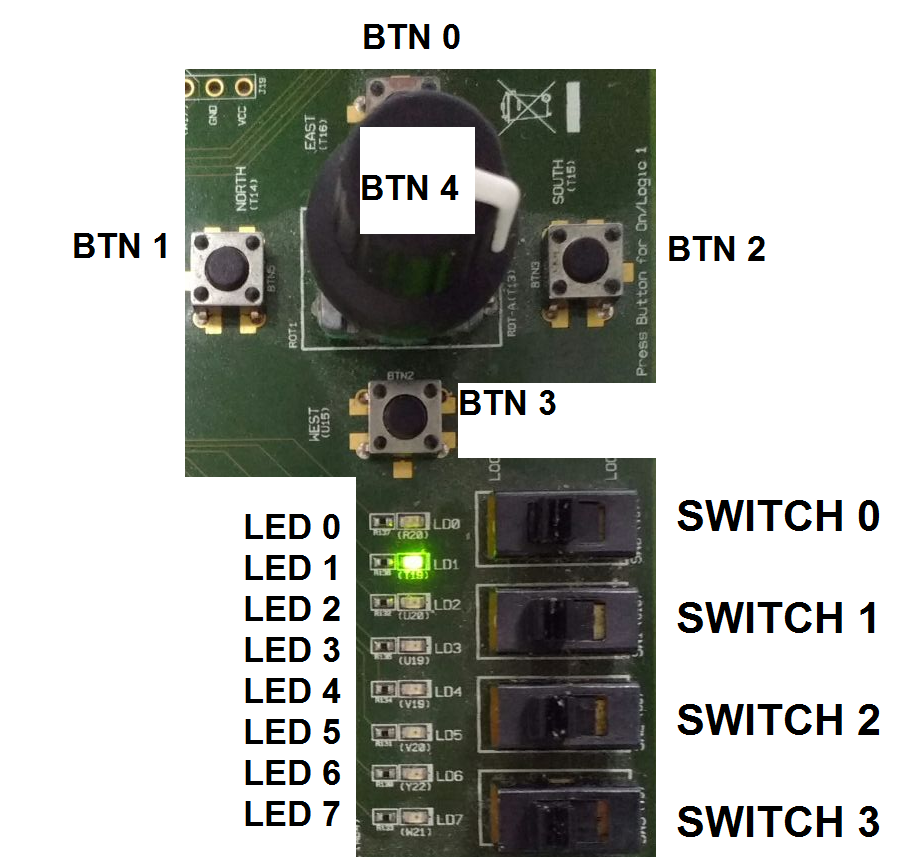
\includegraphics[scale=0.1\textwidth]{pinning.png}
	\caption{Verteilung der I/O-Signale}
	\label{fig:pinning}
\end{figure}


